\section{Sprint 3 conclusion}\label{sec:sprint3conclusion}
This section concludes the preceding chapter on sprint 3.
It will recapitulate the knowledge that was obtained based on the sections of the chapter, and discuss the retrospective meeting that was held in the end of the sprint.

\subsection{Current product}
To give an overview of the progression of the project this section will provide an overview of what has been created during the sprint.
This overview will be split into two categories, to reflect the structure of the project: Networking and game.

\subsubsection{Networking}
The major focus for the network part this sprint was to generate an initial UPPAAL model to visualize the flow of data.
This initial model is based on the assumption that packages are not lost and timeouts will not happen for simplicity.
Creation of this model lead to some revision to the network protocol as described in \autoref{subsec:sprint3networkupdate}.\\
In addition to the UPPAAL model, the ideas behind dead reckoning was examined in relation to this project.
The technique was deemed relevant to implement if the representation of the players' movement is inconsistent, which will be delved further into when the game is connected with the actual Pozyx location data.

\subsubsection{Game}
The most major changes in terms of the game this sprint was the addition of goal zones.
The goal zones were previously generated on the client, but to ensure a consistent game state across all clients, this has been moved to the host and will be transmitted over the network instead.
This meant that the major focus for the game in this sprint was refactoring how goals were displayed, as described in \autoref{subsec:goalrefactoring}.

\begin{figure}[H]
	\centering
	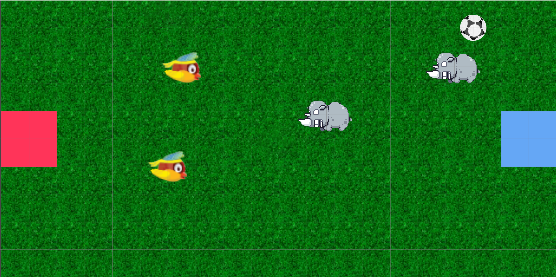
\includegraphics[width=0.6\linewidth]{sprint3/gamestatus.png}
	\caption{The current game status with goals and textures}
	\label{fig:sprint3status}
\end{figure}
\noindent
Additionally, some temporary textures have been added to the game to get rid of the pink playing field and square players.
These new textures can be seen on \autoref{fig:sprint3status}.

\subsection{Retrospective on the process}
The ideal outcome of this sprint was an MVP of the product, but unfortunately, this was not achieved due to various problems.
First of all, there was a series of problems with merge conflicts in auto-generated files in Unity, which lead to the agreement that only one pair of group members should work on Unity at a time to avoid unsolvable merge conflicts.
This lead to a major delay in the Unity development.\\
Additionally, due to the COVID-19 lockdown, we did not have an opportunity to test the system properly with external users to get their feedback on the current product, and what to focus on for the last two sprints.
In addition to discussing the progress of the process, the following points were brought up:

\subsubsection*{How does the process with Jira work?}
The process is generally improved since last time, not having to spend time assigning priority points to every task is nice.
The challenger expressed that he would appreciate if more people contributed to the backlog suggestions since it can be difficult to continuously come up with new tasks.


\subsubsection*{How has pair programming been working?}
It has been good for productivity to have implemented the pair programming practice.
However, it has been hard to coordinate at times, since it requires two people to be free at the same time for a pair programming task to properly start.
In the future, a single person should start with the development and when someone is available to join at a later point, they can.

\subsubsection*{How is the daily stand-up working?}
While the new format proposed in the last sprint's retrospective was effective for a few days, it was quickly forgotten.
To keep the stand-ups effective, the anchor should be better at enforcing that the format is being followed to make sure that we know who needs help, and what people are currently doing.

\subsubsection*{How are the reviews going?}
The pair review format for code does not seem to be working too well since it is usually procrastinated until the next morning because one of the two reviewers is busy with something else.

The single-person reviews are also lacking at the moment, where people do not remember to check what they are assigned to.
It is suggested that people regularly go to the front page of GitHub and check the "Recent Activity" which shows the PRs you are assigned to.
It is also suggested that it is possible to ask people to review your code or text right away if it is important that it gets merged.
This is mostly if the task is blocking other tasks and thus are of great importance.


\subsubsection*{Other comments?}
Finally, we went through all the tasks that had been completed in the sprint to make sure that everything is described in the report.
It worked well, since it helped create an overview of where we are in the project and figure out what to do next.
